\section{Views}
The 'Add View' button \includegraphics[width=0.5cm,frame]{../../data/icons/crosshair_fat.png} on the top right in each window allows adding views to the current window or in a new window. \\

Each View is contained in a tab within a parent window.  At startup, per default only the main window exists, which also holds
a ListBox view. If the main window is closed, the COMPASS client shuts down. New Views can be added using the 'Add View' button, which opens a pull-down menu. Each View can either be added to the main window ('Add Here') or into a new window ('Add in New Window'. When added, a new tab exists in the containing window. \\

New Views can be added either to currently existing windows as new tabs, or to a newly opened window. A window can be closed either by the close button in the window decoration, which discards all contained Views within the window.  \\

To close a single View, one can use the \includegraphics[width=0.5cm,frame]{../../data/icons/edit.png} button in the tab header, which frees up all its allocated resources. \\

Each View adds its required variables to the loading list for the database. During a loading process, the loading status  of a View is shown in the management tab.\\

Currently, the following Views exist:
\begin{itemize}
 \item \nameref{sec:histo_view}
 \item \nameref{sec:listbox_view}
 \item \nameref{sec:osg_view}
 \item \nameref{sec:scatter_view}
\end{itemize}

\subsection{View Presets}

\hl{Each view can be configured to the users needs, to suit various use-cases. For each type of view, a number of pre-defined (default) presets are delivered, which can be used to conveniently set a number of configuration options for specific display purposes. Existing presets can be changed and overridden, also new ones can be created.} \\

In the toolbar of each view, a preset selection dropdown-menu is shown. If clicked, a menu is shown:

\begin{figure}[H]
    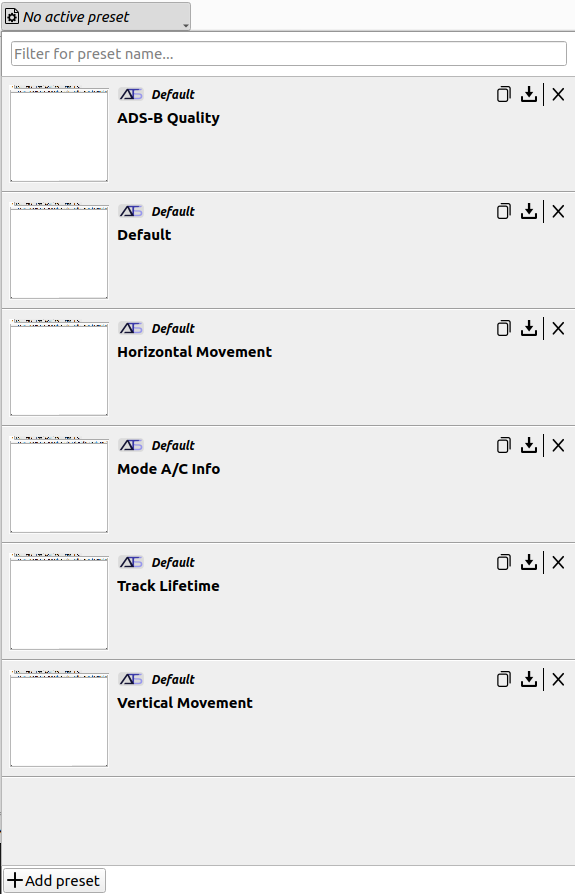
\includegraphics[width=12cm,frame]{figures/view_presets.png}
  \caption{View Preset Selection}
\end{figure}

All existing view presets are listed, and can be selected with a single left click. A preset contains the following information:

\begin{itemize}
 \item Screenshot: A saved screenshot 
 \item Category: Default (delivered with the application) or created by user
 \item Name: A (unique) descriptive name
 \item Description
\end{itemize} \ \\

Additionally, a number of actions exist per preset:

\begin{itemize}
 \item \includegraphics[width=0.5cm,frame]{../../data/icons/edit_old.png}: Edit the preset (name, category, description)
 \item 
\includegraphics[width=0.5cm,frame]{../../data/icons/copy.png}: Copy the preset into a new one
 \item \includegraphics[width=0.5cm,frame]{../../data/icons/save.png}: Save the current changes into the preset
 \item \includegraphics[width=0.5cm,frame]{../../data/icons/delete.png}: Delete the preset
\end{itemize} \ \\

Editing a preset shows the following dialog:

\begin{figure}[H]
    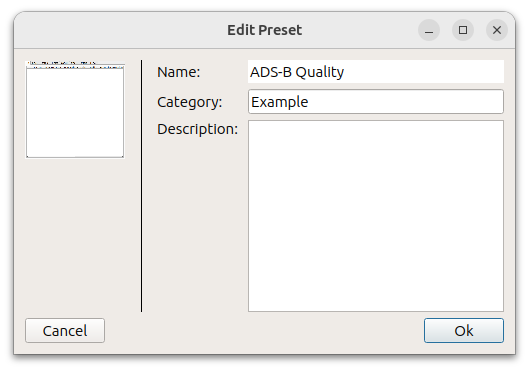
\includegraphics[width=10cm]{figures/view_preset_edit.png}
  \caption{View Preset Editing}
\end{figure}

At the very bottom, a button exists for adding new presets, as for creating a new preset from the current configuration. \\

Please \textbf{note} that if a view preset is selected, the configuration is applied automatically, often triggering a reload of the surveillance data. \\
Also, if changes are made in the configuration tab, these changes are not saved to the preset by default. Such an action as to be performed manually by the user. \\

Please also \textbf{note} that user-created view presets are created per COMPASS version, and have to be created each time a COMPASS version upgrade is performed. If this is cumbersome, or if a view preset was created which should added as a default one, please contact \href{mailto:compass@openats.at}{compass@openats.at} for support.

